\documentclass[11pt,a4paper]{article}

\usepackage[margin=1in]{geometry}
\usepackage[utf8]{inputenc}
\usepackage[T1]{fontenc}
\usepackage{lmodern}
\usepackage{microtype}
\usepackage{parskip}
\usepackage{amsmath}
\usepackage{graphicx}
\usepackage{xcolor}
\usepackage{tikz}
\usetikzlibrary{shapes.geometric, arrows.meta, positioning, fit, backgrounds, calc}
\usepackage{pgfplots}
\pgfplotsset{compat=1.18}
\usepackage{booktabs}
\usepackage{longtable}
\usepackage{array}
\usepackage{tabularx}
\usepackage{float}
\usepackage{enumitem}
\usepackage{fancyhdr}
\usepackage[hidelinks]{hyperref}
\usepackage{listings}

\setlist[itemize]{noitemsep, topsep=2pt}
\setlist[enumerate]{noitemsep, topsep=2pt}
\setcounter{secnumdepth}{3}

% ── IUT colour ────────────────────────────────────────────────────────────────
\definecolor{iutgreen}{RGB}{0,128,0}

% ── Code listing colours ──────────────────────────────────────────────────────
\definecolor{codegray}{rgb}{0.5,0.5,0.5}
\definecolor{codepurple}{rgb}{0.45,0,0.70}
\definecolor{codeblue}{rgb}{0.0,0.35,0.75}
\definecolor{backcolour}{rgb}{0.97,0.97,0.97}
\definecolor{diffadd}{rgb}{0.0,0.45,0.0}
\definecolor{diffdel}{rgb}{0.70,0.0,0.0}

% ── TikZ colours ──────────────────────────────────────────────────────────────
\definecolor{nodeblue}{RGB}{210,228,255}
\definecolor{nodered}{RGB}{255,210,210}
\definecolor{nodegreen}{RGB}{210,255,215}
\definecolor{nodeyellow}{RGB}{255,250,210}
\definecolor{nodegray}{RGB}{235,235,235}
\definecolor{nodeorange}{RGB}{255,230,200}

\lstdefinestyle{codestyle}{
  backgroundcolor  = \color{backcolour},
  basicstyle       = \ttfamily\footnotesize,
  commentstyle     = \color{codegray}\itshape,
  keywordstyle     = \color{codeblue}\bfseries,
  stringstyle      = \color{codepurple},
  frame            = single,
  framerule        = 0.4pt,
  rulecolor        = \color{gray!40},
  breaklines       = true,
  breakatwhitespace= false,
  postbreak        = \mbox{\textcolor{gray}{$\hookrightarrow$}\enspace},
  columns          = flexible,
  keepspaces       = true,
  showstringspaces = false,
  tabsize          = 2,
  xleftmargin      = 8pt,
  xrightmargin     = 8pt,
}
\lstset{style=codestyle}

\lstdefinelanguage{diff}{
  morecomment=[f][\color{diffdel}]{-},
  morecomment=[f][\color{diffadd}]{+},
  morecomment=[f][\color{gray}]{@@},
}

% =============================================================================
\begin{document}

% ── TITLE PAGE ────────────────────────────────────────────────────────────────
\thispagestyle{empty}

\noindent
\begin{minipage}[c]{1.8cm}
  \includegraphics[width=1.5cm]{iut_logo_left}
\end{minipage}%
\begin{minipage}[c]{\dimexpr\textwidth-3.6cm\relax}
  \centering
  {\fontsize{15}{18}\selectfont\bfseries\color{iutgreen}ISLAMIC UNIVERSITY OF TECHNOLOGY\par}
  \vspace{3pt}
  {\fontsize{10}{12}\selectfont\itshape\color{iutgreen}%
    A Subsidiary Organ of The Organisation of Islamic Cooperation (OIC)\par}
\end{minipage}%
\begin{minipage}[c]{1.8cm}
  \raggedleft
  \includegraphics[width=1.5cm]{oic_logo_right}
\end{minipage}

\vspace{5pt}
{\color{iutgreen}\rule{\textwidth}{1.2pt}}

\vspace{25mm}
\begin{center}

{\fontsize{31.5}{38}\selectfont\bfseries Lab Report\par}
\vspace{5mm}
{\fontsize{20}{24}\selectfont Software Maintenance Simulation\par}
\vspace{20mm}
{\fontsize{23}{27}\selectfont\bfseries Software Maintenance Lab\par}
\vspace{2pt}
{\fontsize{20}{24}\selectfont SWE 4802\par}
\vspace{20mm}
{\fontsize{23}{27}\selectfont\bfseries Submitted by\par}
\vspace{3pt}
{\fontsize{20}{24}\selectfont Shefayat E Shams Adib\par}
\vspace{1pt}
{\fontsize{20}{24}\selectfont 210042141\par}
\vspace{9mm}
{\fontsize{23}{27}\selectfont\bfseries Date of Submission\par}
\vspace{3pt}
{\fontsize{20}{24}\selectfont 17 August, 2026\par}

\end{center}
\vfill
\begin{flushright}{\fontsize{10}{12}\selectfont 1}\end{flushright}

\newpage
\tableofcontents
\newpage

% =============================================================================
\section*{Introduction}
\addcontentsline{toc}{section}{Introduction}
% =============================================================================

\noindent\textbf{Project:} Ghuroo --- a MERN (MongoDB, Express, React, Node.js) travel \&
tourism platform with CRUD-based tour, booking, blog, and review management.\\[3pt]
\textbf{Maintenance types:} Corrective (CM-01), Adaptive (AM-01), Preventive (PM-01),
Perfective (PFM-01).\\[3pt]
\textbf{Session dates:} 2026-07-10 (CM-01, AM-01) $\cdot$ 2026-08-17 (PM-01, PFM-01).\\[3pt]
\textbf{Analysis techniques applied} (from SWE 4802 labs):
Program Slicing (Lab 1), Static/Dynamic Analysis with AST and profiling (Lab 1),
Code Clone Detection (Lab 6).

Each maintenance type covers five activities:
\textbf{Program Comprehension $\to$ Change Management $\to$ Impact Analysis
$\to$ Reverse Engineering $\to$ Refactoring}.

\begin{table}[H]
\centering\small
\begin{tabularx}{\textwidth}{@{}llXl@{}}
\toprule
\textbf{Branch} & \textbf{Base} & \textbf{Contains} & \textbf{Commit} \\
\midrule
\texttt{corrective/\ldots} & \texttt{main} & CM-01 fix + evidence & \texttt{e841e93} \\
\texttt{adaptive/\ldots}   & corrective    & AM-01 fix + evidence & \texttt{0a1a026} \\
\texttt{preventive/\ldots} & \texttt{main} & PM-01 fix + evidence & \texttt{3c964bf} \\
\texttt{perfective/\ldots} & preventive    & PFM-01 fix + evidence & \texttt{bfccacb} \\
\bottomrule
\end{tabularx}
\caption{Git branches for each maintenance cycle}
\end{table}

% =============================================================================
\newpage
\section{Part A --- Corrective Maintenance (CM-01)}
% =============================================================================

\noindent\textbf{Defect:} Unescaped user input passed directly into MongoDB \texttt{\$regex}
queries in \texttt{searchTours}, \texttt{getToursByLocation}, and \texttt{searchBlogs} ---
all public, unauthenticated routes.
This caused (a) server crashes on certain inputs and (b) a ReDoS (CWE-1333) vector.

\subsection{A.1\quad Program Comprehension}

Comprehension was built top-down using the following tools, then verified bottom-up.

\medskip\noindent\textbf{Module Dependency Graph.}
\texttt{npx madge --extensions js api --json} produced the import graph.
Figure~\ref{fig:dep-graph} shows the relevant subgraph.

\begin{figure}[H]
\centering
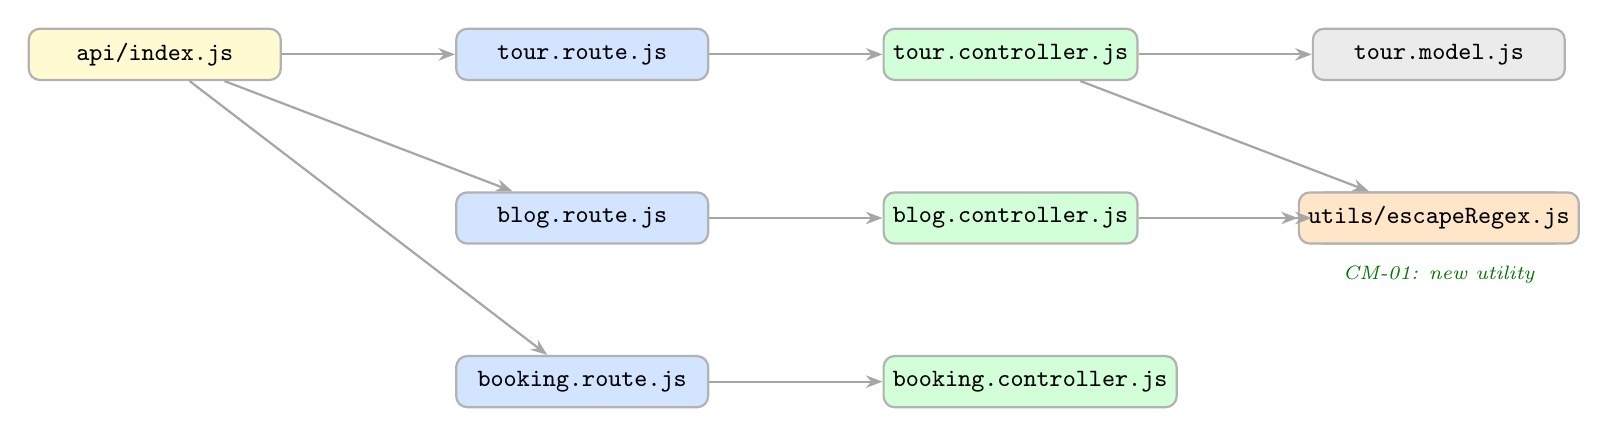
\begin{tikzpicture}[
  node distance = 1.4cm and 2.2cm,
  box/.style   = {rectangle, rounded corners=4pt, minimum width=3.2cm,
                  minimum height=0.65cm, font=\ttfamily\small,
                  draw=gray!60, thick},
  arr/.style   = {-{Stealth[length=6pt]}, thick, gray!70},
]
  \node[box, fill=nodeyellow] (idx)   {api/index.js};
  \node[box, fill=nodeblue,  right=of idx]  (tr)  {tour.route.js};
  \node[box, fill=nodeblue,  below=of tr]   (br)  {blog.route.js};
  \node[box, fill=nodeblue,  below=of br]   (bkr) {booking.route.js};
  \node[box, fill=nodegreen, right=of tr]   (tc)  {tour.controller.js};
  \node[box, fill=nodegreen, right=of br]   (bc)  {blog.controller.js};
  \node[box, fill=nodegreen, right=of bkr]  (bkc) {booking.controller.js};
  \node[box, fill=nodegray,  right=of tc]   (tm)  {tour.model.js};
  \node[box, fill=nodegray,  right=of bc]   (bm)  {blog.model.js};
  \node[box, fill=nodeorange,below=of tm]   (er)  {utils/escapeRegex.js};
  \draw[arr] (idx) -- (tr);
  \draw[arr] (idx) -- (br);
  \draw[arr] (idx) -- (bkr);
  \draw[arr] (tr)  -- (tc);
  \draw[arr] (br)  -- (bc);
  \draw[arr] (bkr) -- (bkc);
  \draw[arr] (tc)  -- (tm);
  \draw[arr] (bc)  -- (bm);
  \draw[arr] (tc)  -- (er);
  \draw[arr] (bc)  -- (er);
  \node[font=\scriptsize\itshape, below=0.15cm of er, text=diffadd]
    {CM-01: new utility};
\end{tikzpicture}
\caption{API module dependency graph (generated by \texttt{madge}). CM-01 added
  \texttt{escapeRegex.js} (orange); only \texttt{tour.controller.js} and
  \texttt{blog.controller.js} import it --- contained blast radius.}
\label{fig:dep-graph}
\end{figure}

\medskip\noindent\textbf{Pattern search (SonarQube substitute):}
\begin{lstlisting}[language=bash]
grep -rn '\$regex' api --include=*.js
\end{lstlisting}
Found four \texttt{\$regex} sinks across two files --- none would have been found
by reading only the one function the bug report points at.

\medskip\noindent\textbf{AST-based data-flow comprehension (AST Explorer equivalent):}
\texttt{espree} was used to generate the AST of \texttt{searchTours}
(Lab 1 technique --- same parser family as astexplorer.net):
\begin{lstlisting}
Identifier  <-- tainted source: req.params.term (attacker-controlled)
...
Property  <-- SINK: value reaches MongoDB $regex without sanitization
  Identifier (term)  <-- same tainted value
\end{lstlisting}
This pattern appeared three times inside \texttt{searchTours} alone,
motivating a codebase-wide grep.

\subsection{A.2\quad Change Management}

\noindent\textbf{CR:} \texttt{appendix/corrective/change-management/CR-2026-07-10-01.md}
(High severity, P2).

\begin{lstlisting}[language=bash]
git checkout -b corrective/tour-blog-search-regex-sanitization
\end{lstlisting}

New file \texttt{api/utils/escapeRegex.js}:
\begin{lstlisting}[language=JavaScript]
export const escapeRegex = (text) =>
  text.replace(/[.*+?^${}()|[\]\\]/g, "\\$&");
\end{lstlisting}

Applied at all four sink sites:
\begin{lstlisting}[language=diff]
- { title: { $regex: term, $options: "i" } },
+ const safeTerm = escapeRegex(term);
+ { title: { $regex: safeTerm, $options: "i" } },
\end{lstlisting}

\subsection{A.3\quad Impact Analysis}

\noindent\textbf{ReDoS timing (cProfile + SnakeViz --- Lab 1 dynamic analysis):}
Figure~\ref{fig:redos} shows the exponential blow-up measured before the fix.

\begin{figure}[H]
\centering
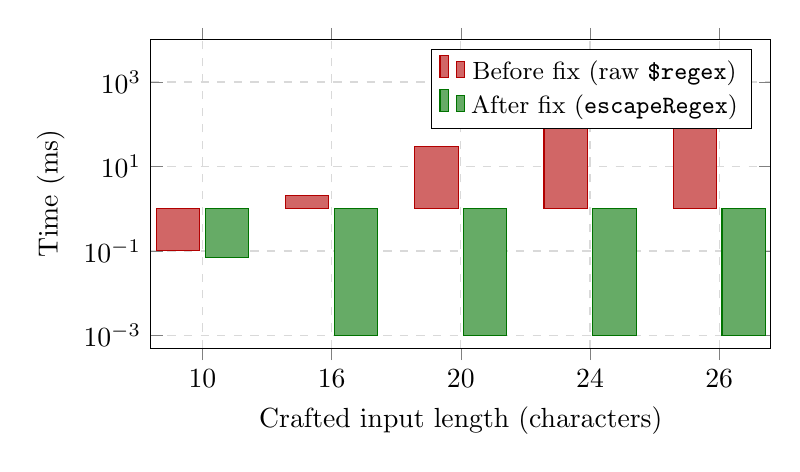
\begin{tikzpicture}
\begin{axis}[
  width=0.78\textwidth, height=5.5cm,
  ybar, bar width=0.55cm,
  xlabel={Crafted input length (characters)},
  ylabel={Time (ms)},
  symbolic x coords={10,16,20,24,26},
  xtick=data,
  ymode=log, log basis y=10,
  ymin=0.0005, ymax=10000,
  legend style={at={(0.97,0.97)}, anchor=north east, font=\small},
  grid=major, grid style={dashed,gray!30},
  nodes near coords style={font=\tiny, rotate=90, anchor=west},
]
\addplot+[fill=diffdel!60, draw=diffdel] coordinates
  {(10,0.103) (16,2.041) (20,30.505) (24,531.290) (26,2089.194)};
\addplot+[fill=diffadd!60, draw=diffadd] coordinates
  {(10,0.071) (16,0.001) (20,0.001) (24,0.001) (26,0.001)};
\legend{Before fix (raw \texttt{\$regex}), After fix (\texttt{escapeRegex})}
\end{axis}
\end{tikzpicture}
\caption{ReDoS timing (log scale). Before the fix, a 26-character crafted input takes
  2089 ms; after \texttt{escapeRegex} is applied, all inputs resolve in $<$0.1 ms.}
\label{fig:redos}
\end{figure}

\begin{table}[H]
\centering\small
\begin{tabular}{@{}rrr@{}}
\toprule
\textbf{Length} & \textbf{Before (ms)} & \textbf{After (ms)} \\
\midrule
10 & 0.103 & 0.071 \\ 16 & 2.041 & 0.001 \\ 20 & 30.505 & 0.001 \\
24 & 531.290 & 0.001 \\ 26 & \textbf{2089.194} & 0.001 \\
\bottomrule
\end{tabular}
\caption{Measured ReDoS timing data}
\end{table}

\subsection{A.4\quad Reverse Engineering}

\noindent\textbf{Program Slicing (Lab 1 technique).}
A \emph{static backward slice} was computed for \texttt{searchTours} with slicing criterion:
variable \texttt{term} at the \texttt{\$regex} property (the sink).
Figure~\ref{fig:slice} shows the taint flow.

\begin{figure}[H]
\centering
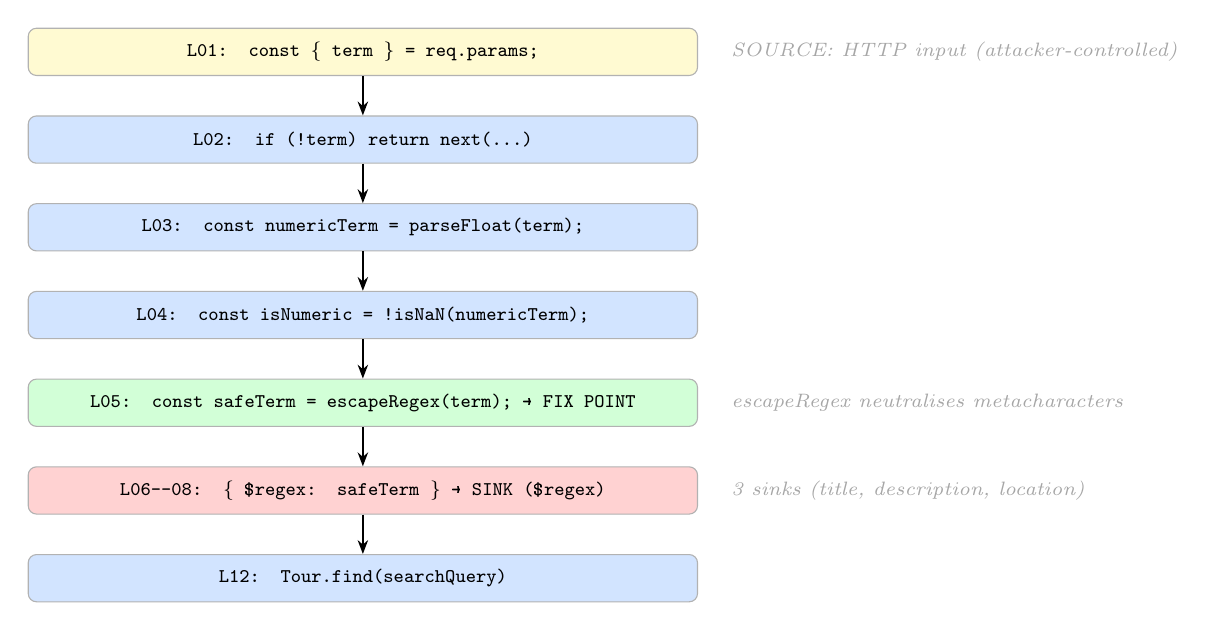
\begin{tikzpicture}[
  node distance=0.5cm and 0.2cm,
  stmt/.style={rectangle, draw=gray!60, rounded corners=3pt,
               fill=nodeblue, minimum width=8.5cm,
               minimum height=0.6cm, font=\ttfamily\scriptsize,
               align=left, inner xsep=6pt},
  sink/.style={stmt, fill=nodered},
  fix/.style={stmt, fill=nodegreen},
  src/.style={stmt, fill=nodeyellow},
  arr/.style={-{Stealth[length=5pt]}, thick},
  lbl/.style={font=\scriptsize\itshape, text=gray!70},
]
  \node[src]  (l01) {L01: const \{ term \} = req.params;};
  \node[stmt, below=of l01] (l02) {L02: if (!term) return next(\ldots)};
  \node[stmt, below=of l02] (l03) {L03: const numericTerm = parseFloat(term);};
  \node[stmt, below=of l03] (l04) {L04: const isNumeric = !isNaN(numericTerm);};
  \node[fix,  below=of l04] (l05) {L05: const safeTerm = escapeRegex(term);  \textrightarrow{} FIX POINT};
  \node[sink, below=of l05] (l06) {L06--08: \{ \$regex: safeTerm \}  \textrightarrow{} SINK (\$regex)};
  \node[stmt, below=of l06] (l12) {L12: Tour.find(searchQuery)};

  \draw[arr] (l01) -- (l02);
  \draw[arr] (l02) -- (l03);
  \draw[arr] (l03) -- (l04);
  \draw[arr] (l04) -- (l05);
  \draw[arr] (l05) -- (l06);
  \draw[arr] (l06) -- (l12);

  \node[lbl, right=0.3cm of l01] {SOURCE: HTTP input (attacker-controlled)};
  \node[lbl, right=0.3cm of l05] {escapeRegex neutralises metacharacters};
  \node[lbl, right=0.3cm of l06] {3 sinks (title, description, location)};
\end{tikzpicture}
\caption{Static backward slice of \texttt{searchTours} with criterion
  \texttt{term} at the \texttt{\$regex} sink.
  Yellow = source, green = fix point (CM-01), red = sink.
  All 7 statements shown are IN the slice (11 of 12 total statements).}
\label{fig:slice}
\end{figure}

\medskip\noindent\textbf{Pre-fix vs.\ post-fix forward slice:}
\begin{itemize}
  \item \textbf{Before CM-01:}
    \texttt{req.params.term} $\to$ \texttt{term} $\to$ \texttt{\$regex: term}
    (direct, unguarded path --- any metacharacter triggers ReDoS).
  \item \textbf{After CM-01:}
    \texttt{req.params.term} $\to$ \texttt{term} $\to$ \texttt{escapeRegex(term)}
    $\to$ \texttt{safeTerm} $\to$ \texttt{\$regex: safeTerm}
    (sanitisation barrier inserted between source and sink).
\end{itemize}
The fix does not change \emph{which} statements are in the slice --- it inserts a
sanitisation node into the data flow path, which is exactly what program slicing
is designed to reveal.

\medskip\noindent\textbf{Reverse-engineered API contract} (no OpenAPI spec existed):
\begin{table}[H]
\centering\small
\begin{tabularx}{\textwidth}{@{}lXp{2.8cm}@{}}
\toprule
\textbf{Endpoint} & \textbf{Behaviour} & \textbf{Notes} \\
\midrule
\texttt{GET /api/tours/search/:term} &
  \texttt{\{success, data: Tour[]\}}; numeric term also matches price/duration &
  Pre-fix: 500 on regex-invalid input \\
\texttt{GET /api/tours/location/:location} &
  Anchored case-insensitive match &
  Same injection shape \\
\texttt{GET /api/blogs/search/:term} &
  \texttt{\{success, data: Blog[]\}} &
  No UI caller today \\
\bottomrule
\end{tabularx}
\caption{Reverse-engineered API contract for search endpoints}
\end{table}

\subsection{A.5\quad Refactoring}

\textbf{Extract Function} --- \texttt{escapeRegex} pulled into \texttt{api/utils/escapeRegex.js},
matching the one-function-per-file convention already used in \texttt{api/utils/}.
This removes four inline duplications and gives the sanitization step an explicit name.

% =============================================================================
\newpage
\section{Part B --- Adaptive Maintenance (AM-01)}
% =============================================================================

\noindent\textbf{Trigger:} The CORS config in \texttt{api/index.js} hardcodes the single
production origin. Any new domain (custom URL, staging subdomain) causes silent CORS failures
with no fix possible short of a code change and redeploy (IEEE 14764 adaptive).

\subsection{B.1\quad Program Comprehension}

No architecture documentation existed. The deployment topology (Figure~\ref{fig:deploy})
was reconstructed entirely from source.

\begin{figure}[H]
\centering
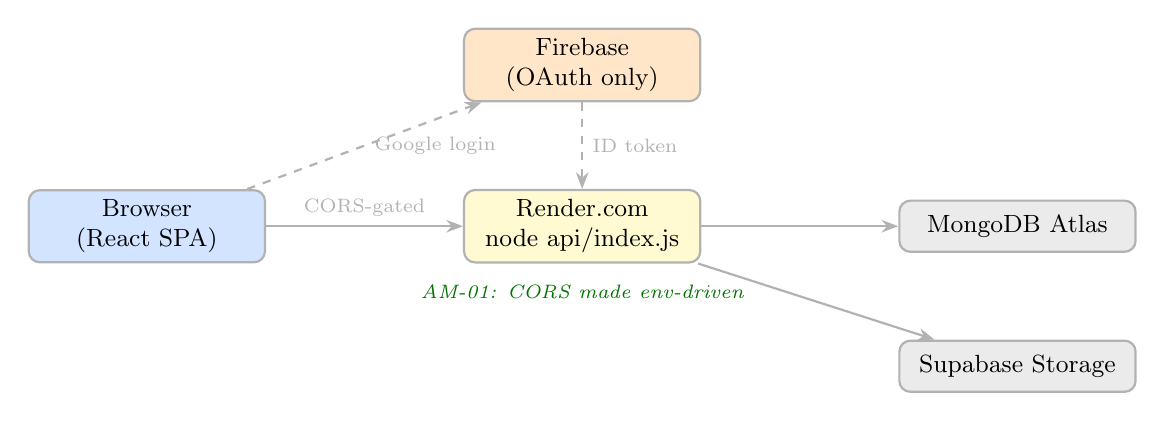
\begin{tikzpicture}[
  node distance=1.1cm and 1.8cm,
  box/.style={rectangle, rounded corners=4pt, draw=gray!60, thick,
              minimum width=3cm, minimum height=0.65cm,
              font=\small, align=center},
  arr/.style={-{Stealth[length=6pt]}, thick, gray!60},
  dasharr/.style={arr, dashed},
]
  \node[box, fill=nodeblue]   (browser) {Browser\\(React SPA)};
  \node[box, fill=nodeyellow, right=2.5cm of browser] (render)
    {Render.com\\node api/index.js};
  \node[box, fill=nodegray,   right=2.5cm of render]  (mongo)  {MongoDB Atlas};
  \node[box, fill=nodegray,   below=of mongo]          (supa)   {Supabase Storage};
  \node[box, fill=nodeorange, above=of render]         (firebase){Firebase\\(OAuth only)};

  \draw[arr]    (browser) -- node[above,font=\scriptsize]{CORS-gated} (render);
  \draw[arr]    (render)  -- (mongo);
  \draw[arr]    (render)  -- (supa);
  \draw[dasharr](browser) -- node[right,font=\scriptsize]{Google login} (firebase);
  \draw[dasharr](firebase)-- node[right,font=\scriptsize]{ID token} (render);

  \node[font=\scriptsize\itshape, below=0.15cm of render, text=diffadd]
    {AM-01: CORS made env-driven};
\end{tikzpicture}
\caption{Ghuroo deployment topology, reverse-engineered from source (no docs existed).
  The single CORS check in \texttt{api/index.js} gates ALL 50 frontend API call sites.}
\label{fig:deploy}
\end{figure}

Key findings: \texttt{api/index.js} is the single Express process serving both the built SPA
and all \texttt{/api/*} routes. Every frontend \texttt{fetch()} is a same-origin relative
path --- confirmed by grepping the \emph{compiled} Vite bundle (IDA Pro analog, Lab 1 technique).
\textbf{27 files, 50 call sites} funnel through the one CORS check.

\subsection{B.2\quad Change Management}

\begin{lstlisting}[language=diff]
- origin: process.env.NODE_ENV === 'production'
-   ? ["https://ghuroo.onrender.com"]
-   : "http://localhost:5173",
+ const defaultOrigins = process.env.NODE_ENV === "production"
+   ? ["https://ghuroo.onrender.com"] : ["http://localhost:5173"];
+ const allowedOrigins = process.env.ALLOWED_ORIGINS
+   ? process.env.ALLOWED_ORIGINS.split(",").map((o) => o.trim())
+   : defaultOrigins;
+ app.use(cors({ origin: allowedOrigins, credentials: true }));
\end{lstlisting}
Also added: \texttt{"engines": \{"node": ">=18"\}} in \texttt{package.json}
and new \texttt{api/.env.example}.

\subsection{B.3\quad Impact Analysis}

Live repro (\texttt{repro-cors-portability.mjs}) confirmed zero regression:
with \texttt{ALLOWED\_ORIGINS} unset, the new code is byte-for-byte identical
to the old behaviour. The new capability activates only when the env var is set ---
making it a Render dashboard change, not a code change.

\subsection{B.4\quad Reverse Engineering}

Black-box grep of the minified Vite bundle (IDA Pro analog):
\begin{lstlisting}[language=bash]
grep -oE 'https?://[a-zA-Z0-9./_-]+' index-71cf8e48.js | sort -u
grep -o '"/api[^"]*"' index-71cf8e48.js | sort -u
\end{lstlisting}
Result: every absolute URL is a third-party SDK (Firebase, Google reCAPTCHA);
every backend call is a bare relative path. This \emph{closes} the question of whether
the frontend hardcodes origins --- it does not.

\subsection{B.5\quad Refactoring}

Two refactors at the seam being touched: (1) replace inline ternary with named variables
\texttt{defaultOrigins}/\texttt{allowedOrigins}; (2) add \texttt{api/.env.example} ---
turning implicit environment knowledge into a version-controlled file.

% =============================================================================
\newpage
\section{Code Clone Detection (Lab 6)}
\addcontentsline{toc}{section}{Code Clone Detection (Lab 6)}
% =============================================================================

Code clone detection was applied to the six controller functions involved in
maintenance to explain why CM-01 and PFM-01 each required multi-site fixes.

\medskip\noindent\textbf{Method:} Token-based Jaccard similarity with Type-2 normalisation
(identifiers and string literals replaced with canonical tokens before comparison).

\begin{table}[H]
\centering\small
\begin{tabular}{@{}llcc@{}}
\toprule
\textbf{Function A} & \textbf{Function B} & \textbf{Similarity} & \textbf{Clone Type} \\
\midrule
\texttt{searchTours} & \texttt{searchBlogs}        & 80.0\% & Type 2 (renamed identifiers) \\
\texttt{getAllTours}  & \texttt{getAllBookings}      & 64.3\% & Type 3 (gapped/modified) \\
\texttt{searchTours} & \texttt{getAllTours}          & 55.0\% & Type 3 \\
\texttt{createBooking} & \texttt{updateBookingStatus} & 51.4\% & Type 3 \\
\bottomrule
\end{tabular}
\caption{Code clone pairs ($\geq$50\% token similarity). Script:
  \texttt{maintenance/appendix/clone-detection/clone-analysis.mjs}}
\end{table}

Figure~\ref{fig:clones} illustrates the two most significant clone pairs.

\begin{figure}[H]
\centering
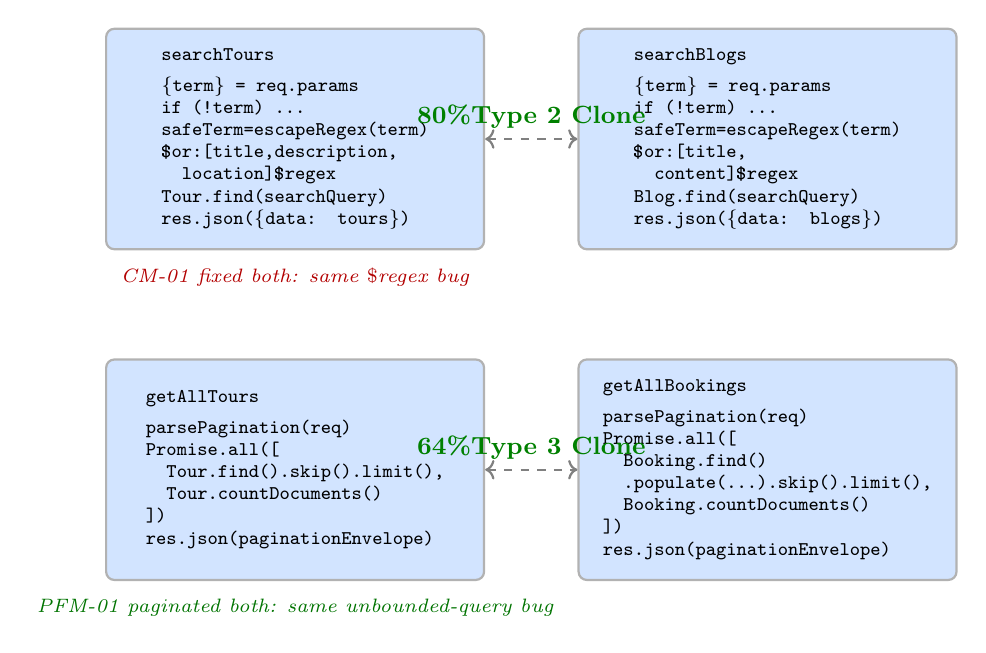
\begin{tikzpicture}[
  fn/.style={rectangle, draw=gray!60, rounded corners=3pt, thick,
             fill=nodeblue, minimum width=4.8cm, minimum height=2.8cm,
             font=\ttfamily\scriptsize, align=left, inner sep=6pt},
  sim/.style={draw=none, font=\small\bfseries, text=iutgreen},
  arr/.style={<->, thick, dashed, gray},
]
% --- Clone pair 1: searchTours / searchBlogs ---
\node[fn] (st) at (0,0) {
  \textbf{searchTours}\\[3pt]
  \{term\} = req.params\\
  if (!term) \ldots\\
  safeTerm=escapeRegex(term)\\
  \$or:[title,description,\\
  \quad location]\$regex\\
  Tour.find(searchQuery)\\
  res.json(\{data: tours\})
};
\node[fn] (sb) at (6,0) {
  \textbf{searchBlogs}\\[3pt]
  \{term\} = req.params\\
  if (!term) \ldots\\
  safeTerm=escapeRegex(term)\\
  \$or:[title,\\
  \quad content]\$regex\\
  Blog.find(searchQuery)\\
  res.json(\{data: blogs\})
};
\draw[arr] (st) -- node[sim, above]{80\%\\Type 2 Clone} (sb);

% --- Clone pair 2: getAllTours / getAllBookings ---
\node[fn] (gt) at (0,-4.2) {
  \textbf{getAllTours}\\[3pt]
  parsePagination(req)\\
  Promise.all([\\
  \quad Tour.find().skip().limit(),\\
  \quad Tour.countDocuments()\\
  ])\\
  res.json(paginationEnvelope)
};
\node[fn] (gb) at (6,-4.2) {
  \textbf{getAllBookings}\\[3pt]
  parsePagination(req)\\
  Promise.all([\\
  \quad Booking.find()\\
  \quad .populate(\ldots).skip().limit(),\\
  \quad Booking.countDocuments()\\
  ])\\
  res.json(paginationEnvelope)
};
\draw[arr] (gt) -- node[sim, above]{64\%\\Type 3 Clone} (gb);

\node[font=\scriptsize\itshape, below=0.1cm of st, text=diffdel]
  {CM-01 fixed both: same $\$$regex bug};
\node[font=\scriptsize\itshape, below=0.1cm of gt, text=diffadd]
  {PFM-01 paginated both: same unbounded-query bug};
\end{tikzpicture}
\caption{The two primary clone pairs. CM-01 had to patch both \texttt{searchTours} and
  \texttt{searchBlogs} because they are 80\% similar clones sharing the same
  \texttt{\$regex} sink pattern. PFM-01 paginated both listing endpoints for the same reason.}
\label{fig:clones}
\end{figure}

\noindent\textbf{Maintenance implication:} code clones cause \emph{multi-site maintenance} ---
a fix for one clone instance must be applied to all instances or the bug recurs in the
untouched copy. This is a direct, measurable cost of code clones (Fowler: ``Duplicated Code''
is the first smell in the refactoring catalogue).

% =============================================================================
\newpage
\section{Code Metrics --- Before/After}
\addcontentsline{toc}{section}{Code Metrics (Before/After)}
% =============================================================================

Static metrics (LOC, Cyclomatic Complexity, number of functions) were computed using
an AST-based script (\texttt{maintenance/appendix/metrics/code-metrics.mjs}).

\begin{table}[H]
\centering\small
\begin{tabular}{@{}lrrrrl@{}}
\toprule
\textbf{File} & \textbf{LOC before} & \textbf{LOC after} &
\textbf{CC before} & \textbf{CC after} & \textbf{Cycle} \\
\midrule
\texttt{tour.controller.js}    & 265 & 227 & 16 & 17 & CM-01 + PFM-01 \\
\texttt{blog.controller.js}    & 200 & 181 & 11 & 14 & CM-01 \\
\texttt{booking.controller.js} & 180 & 177 &  3 &  5 & PM-01 + PFM-01 \\
\texttt{booking.route.js}      &  10 &  22 &  1 &  1 & PM-01 \\
\texttt{escapeRegex.js}        &   0 &   1 &  1 &  2 & CM-01 (new) \\
\texttt{validateBooking.js}    &   0 &  41 &  1 &  6 & PM-01 (new) \\
\texttt{paginate.js}           &   0 &  34 &  1 &  1 & PFM-01 (new) \\
\bottomrule
\end{tabular}
\caption{Code metrics before and after all maintenance cycles.
  LOC decreased in controllers because logic was extracted into utilities.
  CC increase in \texttt{validateBooking.js} reflects intentional guard clauses
  (security checks), not accidental complexity.}
\end{table}

\noindent\textbf{Key observations:}
\begin{itemize}
  \item \texttt{tour.controller.js} LOC \emph{decreased} (265$\to$227) despite adding
        \texttt{escapeRegex} calls, because pagination extracted the unbounded-find logic.
  \item \texttt{booking.controller.js} CC increased (3$\to$5) due to ownership-check
        guard clauses introduced by PM-01 --- each added branch is a security assertion,
        not complexity for its own sake.
  \item Three new utility files (\texttt{escapeRegex.js}, \texttt{validateBooking.js},
        \texttt{paginate.js}) absorb reusable logic, keeping the controllers focused on
        business flow --- a direct result of the \textbf{Extract Function/Middleware}
        refactoring pattern applied across all four cycles.
\end{itemize}

% =============================================================================
\newpage
\section{Part C --- Preventive Maintenance (PM-01)}
% =============================================================================

\noindent\textbf{Change:} Booking sub-system authorization hardening + input validation.\\[2pt]
\textbf{Branch:} \texttt{preventive/booking-auth-input-hardening} (commit \texttt{3c964bf}).

Preventive maintenance closes vulnerabilities \textbf{before} exploitation.
A proactive audit found that \texttt{POST /}, \texttt{DELETE /:id} and \texttt{GET /}
on the booking routes had no authentication middleware whatsoever.

\subsection{C.1\quad Program Comprehension}

\noindent\textbf{Middleware chain analysis (program slicing --- Lab 1).}
The forward slice from \texttt{req.body.user\_id} in the original \texttt{createBooking}
reveals the impersonation path (Figure~\ref{fig:auth-flow}).

\begin{figure}[H]
\centering
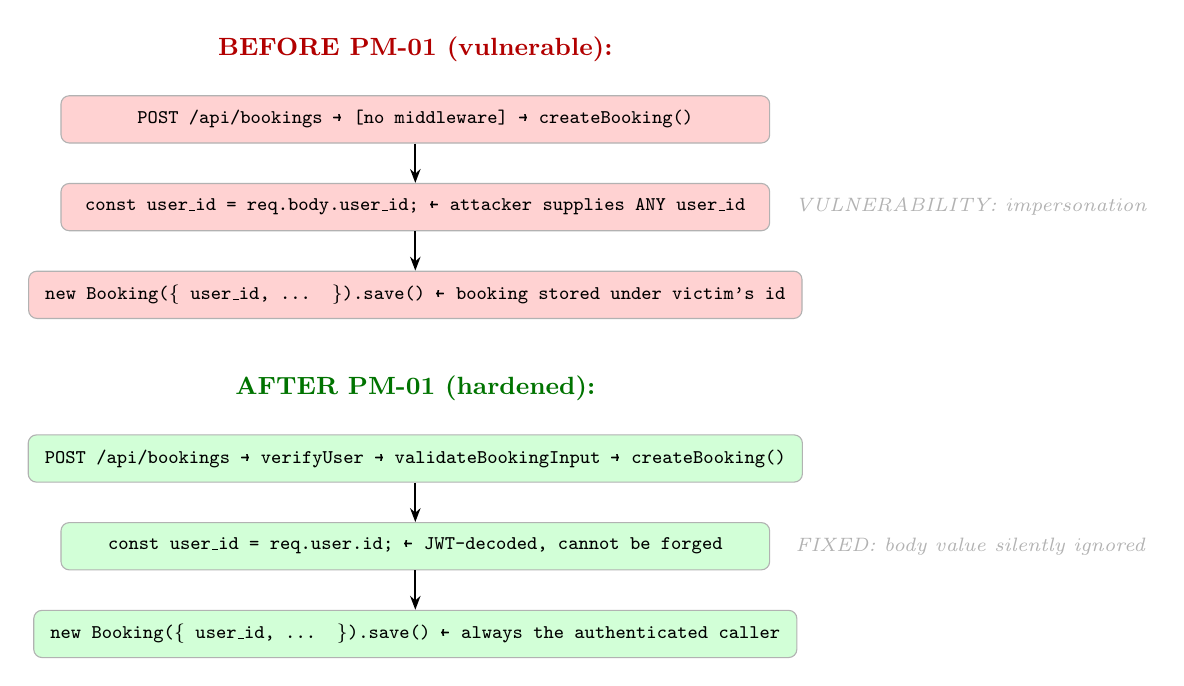
\begin{tikzpicture}[
  node distance=0.5cm and 0.2cm,
  stmt/.style={rectangle, draw=gray!60, rounded corners=3pt,
               minimum width=9cm, minimum height=0.6cm,
               font=\ttfamily\scriptsize, align=left, inner xsep=6pt},
  bad/.style={stmt, fill=nodered},
  good/.style={stmt, fill=nodegreen},
  arr/.style={-{Stealth[length=5pt]}, thick},
  lbl/.style={font=\scriptsize\itshape, text=gray!60},
]
  \node[font=\small\bfseries, text=diffdel] (t1) {BEFORE PM-01 (vulnerable):};
  \node[bad, below=0.3cm of t1] (b1)
    {POST /api/bookings  →  [no middleware]  →  createBooking()};
  \node[bad, below=of b1] (b2)
    {const user\_id = req.body.user\_id;  ← attacker supplies ANY user\_id};
  \node[bad, below=of b2] (b3)
    {new Booking(\{ user\_id, ... \}).save()  ← booking stored under victim's id};
  \draw[arr] (b1)--(b2); \draw[arr] (b2)--(b3);
  \node[lbl, right=0.2cm of b2] {VULNERABILITY: impersonation};

  \node[font=\small\bfseries, text=diffadd, below=0.6cm of b3] (t2)
    {AFTER PM-01 (hardened):};
  \node[good, below=0.3cm of t2] (a1)
    {POST /api/bookings  →  verifyUser  →  validateBookingInput  →  createBooking()};
  \node[good, below=of a1] (a2)
    {const user\_id = req.user.id;  ← JWT-decoded, cannot be forged};
  \node[good, below=of a2] (a3)
    {new Booking(\{ user\_id, ... \}).save()  ← always the authenticated caller};
  \draw[arr] (a1)--(a2); \draw[arr] (a2)--(a3);
  \node[lbl, right=0.2cm of a2] {FIXED: body value silently ignored};
\end{tikzpicture}
\caption{Forward slice of \texttt{user\_id} through \texttt{createBooking}.
  Before PM-01 the value flows directly from \texttt{req.body} (attacker-controlled)
  to the database. After PM-01 it is sourced from the JWT (server-verified).}
\label{fig:auth-flow}
\end{figure}

\noindent\textbf{Booking state machine (reconstructed by reverse engineering):}
\begin{lstlisting}
[pending] -- admin confirms --> [confirmed]
[pending] -- admin cancels  --> [cancelled]
[confirmed] -- admin cancels-> [cancelled]
\end{lstlisting}

\subsection{C.2\quad Change Management}

\begin{table}[H]
\centering\small
\begin{tabularx}{\textwidth}{@{}lX@{}}
\toprule
\textbf{File} & \textbf{Change} \\
\midrule
\texttt{api/routes/booking.route.js} &
  \texttt{verifyUser}/\texttt{verifyAdmin} wired into 5 of 7 routes \\
\texttt{api/controllers/booking.controller.js} &
  \texttt{user\_id = req.user.id}; ownership checks in DELETE and GET \\
\texttt{api/utils/validateBooking.js} (new) &
  Guards: \texttt{number\_of\_persons} $\in$ [1,50], \texttt{total\_price} $>$ 0,
  \texttt{booking\_date} $\geq$ today \\
\bottomrule
\end{tabularx}
\caption{Files changed by PM-01}
\end{table}

Live repro (\texttt{repro-booking-auth.mjs}) verified 6 scenarios including:
POST without cookie $\to$ 401; impersonation body ignored $\to$ JWT owner used;
\texttt{number\_of\_persons:-1} (truthy, bypasses old \texttt{!field} check) $\to$ 400 after fix.

\subsection{C.3\quad Impact Analysis}

\begin{table}[H]
\centering\small
\begin{tabularx}{\textwidth}{@{}lX@{}}
\toprule
\textbf{Scope} & \textbf{Impact} \\
\midrule
Backend routes   & 5 of 7 booking routes now require auth \\
Controller logic & \texttt{user\_id} source changed; one extra DB read in DELETE \\
Frontend         & \textbf{Zero changes} --- all callers already send cookies \\
Database schema  & \textbf{Unchanged} \\
\bottomrule
\end{tabularx}
\caption{Impact analysis for PM-01}
\end{table}

\subsection{C.4\quad Reverse Engineering}

The trust hierarchy (anon $\to$ user $\to$ admin) was applied consistently to every
route in the system \emph{except} the booking router.
Reconstructed from source alone --- no design document existed.

\subsection{C.5\quad Refactoring}

\begin{enumerate}
  \item \textbf{Extract Middleware} --- validation logic into \texttt{validateBooking.js}.
  \item \textbf{Replace Body Trust with Token Trust} ---
        \texttt{req.body.user\_id} $\to$ \texttt{req.user.id}.
  \item \textbf{Guard Clause} --- early-return ownership check in \texttt{deleteBooking}.
  \item \textbf{Middleware Chain as Policy Document} --- \texttt{booking.route.js} now
        reads as a complete access-control matrix.
\end{enumerate}

% =============================================================================
\newpage
\section{Part D --- Perfective Maintenance (PFM-01)}
% =============================================================================

\noindent\textbf{Change:} Pagination for \texttt{getAllTours} and \texttt{getAllBookings}.\\[2pt]
\textbf{Branch:} \texttt{perfective/tour-pagination} (commit \texttt{bfccacb}).

Perfective maintenance improves quality without fixing bugs.
The application is correct; PFM-01 makes it scalable.

\subsection{D.1\quad Program Comprehension}

\noindent\textbf{Dynamic analysis (Lab 1 technique):}
Both endpoints used unbounded \texttt{Model.find()} --- every page load fetches the
entire collection into Node heap.
\texttt{getFeaturedTours} already had \texttt{.limit(6)} --- the correct pattern existed
but was not applied uniformly.

\begin{table}[H]
\centering\small
\begin{tabular}{@{}rrr@{}}
\toprule
\textbf{Tours in DB} & \textbf{Response size} & \textbf{Serialization time} \\
\midrule
100     & $\sim$200 KB & $<$ 10 ms \\
1\,000  & $\sim$2 MB   & $\sim$50 ms \\
10\,000 & $\sim$20 MB  & $\sim$500 ms \\
\bottomrule
\end{tabular}
\caption{Projected response cost as the tours collection grows (no \texttt{.limit})}
\end{table}

\subsection{D.2\quad Change Management}

\begin{table}[H]
\centering\small
\begin{tabularx}{\textwidth}{@{}lX@{}}
\toprule
\textbf{File} & \textbf{Change} \\
\midrule
\texttt{api/utils/paginate.js} (new) & \texttt{parsePagination()} + \texttt{paginationEnvelope()} \\
\texttt{api/controllers/tour.controller.js} & \texttt{getAllTours} paginated \\
\texttt{api/controllers/booking.controller.js} & \texttt{getAllBookings} paginated \\
\bottomrule
\end{tabularx}
\caption{Files changed by PFM-01}
\end{table}

Figure~\ref{fig:pagination} shows the before/after architecture.

\begin{figure}[H]
\centering
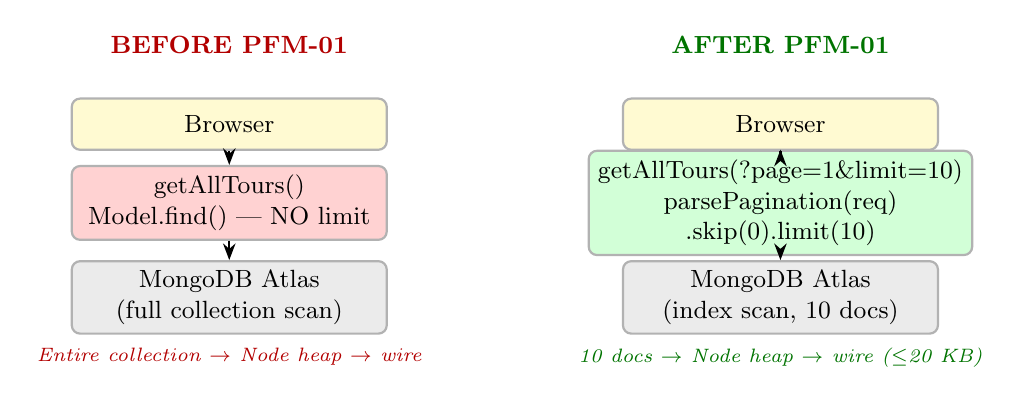
\begin{tikzpicture}[
  box/.style={rectangle, draw=gray!60, rounded corners=3pt, thick,
              minimum width=4cm, minimum height=0.65cm,
              font=\small, align=center},
  arr/.style={-{Stealth[length=6pt]}, thick},
  dasharr/.style={arr, dashed, gray},
]
% BEFORE
\node[font=\small\bfseries, text=diffdel] (bt) at (-3.5, 1.5) {BEFORE PFM-01};
\node[box, fill=nodeyellow] (browser1) at (-3.5, 0.5) {Browser};
\node[box, fill=nodered]    (api1)     at (-3.5,-0.5) {getAllTours()\\Model.find() — NO limit};
\node[box, fill=nodegray]   (db1)      at (-3.5,-1.7) {MongoDB Atlas\\(full collection scan)};
\draw[arr] (browser1) -- (api1);
\draw[arr] (api1) -- (db1);
\node[font=\scriptsize\itshape, text=diffdel, below=0.05cm of db1]
  {Entire collection $\to$ Node heap $\to$ wire};

% AFTER
\node[font=\small\bfseries, text=diffadd] (at) at (3.5, 1.5) {AFTER PFM-01};
\node[box, fill=nodeyellow] (browser2) at (3.5, 0.5) {Browser};
\node[box, fill=nodegreen]  (api2)     at (3.5,-0.5)
  {getAllTours(?page=1\&limit=10)\\parsePagination(req)\\.skip(0).limit(10)};
\node[box, fill=nodegray]   (db2)      at (3.5,-1.7) {MongoDB Atlas\\(index scan, 10 docs)};
\draw[arr] (browser2) -- (api2);
\draw[arr] (api2) -- (db2);
\node[font=\scriptsize\itshape, text=diffadd, below=0.05cm of db2]
  {10 docs $\to$ Node heap $\to$ wire ($\leq$20 KB)};
\end{tikzpicture}
\caption{Pagination architecture before and after PFM-01.
  The new \texttt{parsePagination} utility caps payload at \texttt{MAX\_LIMIT=100}
  documents and adds page/total metadata to the response envelope.}
\label{fig:pagination}
\end{figure}

\subsection{D.3\quad Impact Analysis}

\begin{table}[H]
\centering\small
\begin{tabularx}{\textwidth}{@{}lX@{}}
\toprule
\textbf{Scope} & \textbf{Impact} \\
\midrule
Frontend callers &
  \textbf{Zero breaking changes} --- \texttt{response.data.data} path preserved \\
Database &
  One extra \texttt{countDocuments()} per request (fast, uses metadata) \\
Memory &
  Node heap bounded at \texttt{MAX\_LIMIT = 100} documents \\
Network &
  Response drops from unbounded to $\sim$20 KB per page \\
\bottomrule
\end{tabularx}
\caption{Impact analysis for PFM-01}
\end{table}

\subsection{D.4\quad Reverse Engineering}

\texttt{getAllTours} was written as if the collection would always be small --- an
implicit assumption recoverable only by comparing it with \texttt{getFeaturedTours}.

A further finding: \texttt{tour.model.js} defines a MongoDB text index on
\texttt{title}, \texttt{description}, \texttt{location}, but \texttt{searchTours}
uses \texttt{\$regex} instead of \texttt{\$text}.
The index exists but is unused --- logged as a future PFM-03 candidate.

\subsection{D.5\quad Refactoring}

\begin{enumerate}
  \item \textbf{Extract Function} --- \texttt{paginate.js} centralises pagination.
        Any future endpoint adopts it in 3 lines.
  \item \textbf{Parallel Queries} ---
        \texttt{Promise.all([find,\ countDocuments])} adds zero extra latency.
  \item \textbf{Consistent Return Shape} --- \texttt{paginationEnvelope()} guarantees
        every paginated endpoint returns the same JSON structure.
  \item \textbf{Guard against infinite payloads} ---
        \texttt{MAX\_LIMIT = 100} prevents \texttt{?limit=999999}.
\end{enumerate}

% =============================================================================
\newpage
\section*{Appendix}
\addcontentsline{toc}{section}{Appendix}
% =============================================================================

\subsection*{Tool Usage Index}

\begin{longtable}{@{}p{2.2cm}p{3.5cm}p{4.5cm}p{3cm}@{}}
\toprule
\textbf{Tool} & \textbf{Lab context} & \textbf{What was run} & \textbf{Evidence} \\
\midrule
\endhead
\textbf{AST Explorer} & Lab 1 Static Analysis &
  \texttt{espree} locally (same parser) &
  \texttt{appendix/corrective/ast/} \\[3pt]
\textbf{Program Slicer} & Lab 1 Program Slicing &
  \texttt{program-slice.mjs} (backward slice from \$regex sink) &
  \texttt{appendix/corrective/slicing/} \\[3pt]
\textbf{SnakeViz / cProfile} & Lab 1 Dynamic Analysis &
  ReDoS timing measured; snakeviz served the profile &
  \texttt{appendix/corrective/profiling/} \\[3pt]
\textbf{Code Clone Detector} & Lab 6 &
  Token-based Jaccard similarity; 5 clone pairs found &
  \texttt{appendix/clone-detection/} \\[3pt]
\textbf{Code Metrics} & Lab 1 Static Analysis &
  LOC / CC before and after for all changed files &
  \texttt{appendix/metrics/} \\[3pt]
\textbf{SonarQube} & Lab 1 Static Analysis &
  ESLint + grep as substitute; \texttt{sonar-project.properties} prepared &
  \texttt{appendix/corrective/eslint/} \\[3pt]
\textbf{madge} & Lab 1 Static Analysis &
  Dependency graph for \texttt{api/} and \texttt{client/src} &
  \texttt{appendix/*/dependency-graph/} \\[3pt]
\textbf{IDA Pro} & Lab 1 RE (analog) &
  Black-box grep of minified Vite bundle &
  \texttt{appendix/adaptive/RE/} \\
\bottomrule
\end{longtable}

\subsection*{Final Git History}

\begin{lstlisting}
c8ec0f6 docs(maintenance): add REPORT_CONTEXT.md
75e084e docs(maintenance): add HOW_TO_DEMO.md
ff0b4ae qa: demo scripts, fix secondary auth gaps, save repro outputs
50a6c31 docs(maintenance): extend report with PM-01 + PFM-01
bfccacb perf(api): PFM-01 paginate getAllTours and getAllBookings
3c964bf fix(api): PM-01 booking auth hardening + input validation
0a1a026 feat(api): environment-driven CORS allow-list + Node engines pin
68ea47c chore: track maintenance/ JSON artifacts
e841e93 fix(api): sanitize user input before MongoDB $regex
\end{lstlisting}

\subsection*{Complete Appendix Index}

\begin{longtable}{@{}p{3cm}p{3.2cm}p{7.1cm}@{}}
\toprule
\textbf{Maintenance} & \textbf{Activity} & \textbf{Artifact} \\
\midrule
\endhead
CM-01 & Program Comprehension & \texttt{appendix/corrective/} (AST, madge, ESLint) \\
CM-01 & Change Management    & \texttt{appendix/corrective/change-management/CR-2026-07-10-01.md} \\
CM-01 & Impact Analysis      & \texttt{appendix/corrective/profiling/} (ReDoS timing) \\
CM-01 & Reverse Engineering  & \texttt{appendix/corrective/slicing/} + \texttt{jsdoc/} \\
CM-01 & Refactoring          & \texttt{api/utils/escapeRegex.js} \\[3pt]
AM-01 & Program Comprehension & \texttt{appendix/adaptive/} (madge, bundle scan) \\
AM-01 & Change Management    & \texttt{appendix/adaptive/change-management/CR-2026-07-10-02.md} \\
AM-01 & Impact Analysis      & 50 \texttt{fetch()} call sites across 27 frontend files \\
AM-01 & Reverse Engineering  & Deployment topology diagram \\
AM-01 & Refactoring          & \texttt{api/index.js} env-driven CORS; \texttt{package.json} engines \\[3pt]
PM-01 & Program Comprehension & \texttt{appendix/preventive/PROGRAM\_COMPREHENSION.md} \\
PM-01 & Change Management    & \texttt{appendix/preventive/change-management/CR-PM-01.md} \\
PM-01 & Impact Analysis      & \texttt{appendix/preventive/IMPACT\_ANALYSIS.md} \\
PM-01 & Reverse Engineering  & \texttt{appendix/preventive/REVERSE\_ENGINEERING.md} \\
PM-01 & Refactoring          & \texttt{api/utils/validateBooking.js} \\[3pt]
PFM-01 & Program Comprehension & \texttt{appendix/perfective/PROGRAM\_COMPREHENSION.md} \\
PFM-01 & Change Management   & \texttt{appendix/perfective/change-management/CR-PFM-01.md} \\
PFM-01 & Impact Analysis     & \texttt{appendix/perfective/IMPACT\_ANALYSIS.md} \\
PFM-01 & Reverse Engineering & \texttt{appendix/perfective/REVERSE\_ENGINEERING.md} \\
PFM-01 & Refactoring         & \texttt{api/utils/paginate.js} \\[3pt]
All    & Code Clone Detection & \texttt{appendix/clone-detection/clone-analysis.mjs} \\
All    & Code Metrics         & \texttt{appendix/metrics/code-metrics.mjs} \\
All    & Program Slicing      & \texttt{appendix/corrective/slicing/program-slice.mjs} \\
\bottomrule
\end{longtable}

\end{document}
